\documentclass[a4paper]{report}
\pagestyle{headings}
\usepackage{hyperref}
\usepackage{listings}
\usepackage{graphicx}
\lstset{language=bash}
\lstset{numbers=right}
\lstset{breaklines}
\title{Lab Report for Object-oriented Programming course \newline
 Lab 2: C/C++ Preprocessor}
\author{Wang, Chen \\ 16307110064 \\ School of Software\\ Fudan University}
\date{\today}
\bibliographystyle{plain}
\begin{document}
\maketitle

\tableofcontents

\chapter{Background Knowledge \& Concepts Required for This Lab}
\section{C/C++ Compiling Process}

\subsection{Overall process of compiling}
Compiling a source code file in C++ is a four-step process.\footnote{ \url{http://faculty.cs.niu.edu/mcmahon/CS241/Notes/compile.html}}
 For example, if you have a C++ source code file named \emph{prog1.cpp} and you execute the compile command
 \begin{lstlisting}[language=bash]
g++ -Wall -std=c++11 -o prog1 prog1.cpp
\end{lstlisting}
the compilation process looks like this:
\begin{enumerate}
\item
The C++ preprocessor copies the contents of the included header files into the source code file, generates macro code, and replaces symbolic constants defined using \emph{\#define} with their values.
\item
The expanded source code file produced by the C++ preprocessor is compiled into the assembly language for the platform.
\item
The assembler code generated by the compiler is assembled into the object code for the platform.
\item
The object code file generated by the assembler is linked together with the object code files for any library functions used to produce an executable file.
\end{enumerate}
By using appropriate compiler options, we can stop this process at any stage.
\begin{enumerate}
\item
To stop the process after the preprocessor step, you can use the \emph{-E} option:
\begin{lstlisting}[language=bash]
g++ -Wall -std=c++11 -E prog1.cpp
\end{lstlisting}

The expanded source code file will be printed on standard output (the screen by default); you can redirect the output to a file if you wish. Note that the expanded source code file is often incredibly large - a 20 line source code file can easily produce an expanded file of 20,000 lines or more, depending on which header files were included.
\item
To stop the process after the compile step, you can use the \emph{-S} option:

\begin{lstlisting}[language=bash]
g++ -Wall -std=c++11 -S prog1.cpp
\end{lstlisting}

By default, the assembler code for a source file named \emph{filename.cpp} will be placed in a file named \emph{filename.s}.
\item
To stop the process after the assembly step, you can use the \emph{-c} option:
\begin{lstlisting}[language=bash]
g++ -Wall -std=c++11 -c prog1.cpp
\end{lstlisting}

By default, the assembler code for a source file named \emph{filename.cpp} will be placed in a file named \emph{filename.o}.
The entire process for compiling is shown in the figure \ref{1}
\begin{figure}
  \centering
  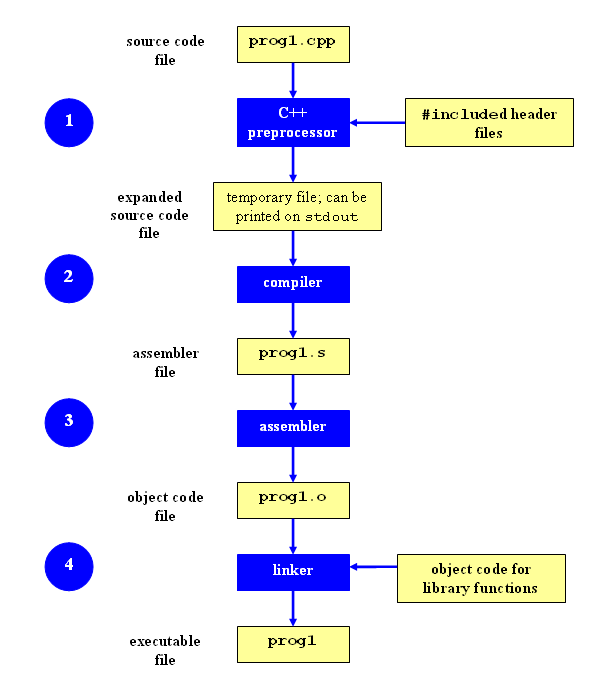
\includegraphics[width=12cm]{compile.png}
  \caption{Overall compiling process}\label{1}
\end{figure}
\end{enumerate}

\subsection{Preprocessing}
To program in C and C++, you need to understand the steps and tools in the compilation process. Some languages (C and C++, in particular) start compilation by running a \emph{preprocessor} on the source code. The preprocessor is a simple program that replaces patterns in the source code with other patterns the programmer has defined (using \emph{preprocessor directives}). Preprocessor directives are used to save typing and to increase the readability of the code. However, from the author of the book TIC, the design of C++ is meant to discourage much of the use of the preprocessor, since it can cause subtle bugs. The pre-processed code is often written to an intermediate file. 
\subsection{Parsing}
Compilers usually do their work in two passes. The first pass \emph{parses} the pre-processed code. The compiler breaks the source code into small units and organizes it into a structure called a \emph{tree}. In the expression “\textbf{A + B}” the elements ‘\textbf{A}’, ‘\textbf{+},’ and ‘\textbf{B}’ are leaves on the parse tree. 
\subsection{Global optimization}
A \emph{global optimizer} is sometimes used between the first and second passes to produce smaller, faster code. 
\subsection{Code generation}
In the second pass, the \emph{code generator} walks through the parse tree and generates either assembly language code or machine code for the nodes of the tree. If the code generator creates assembly code, the assembler must then be run. The end result in both cases is an object module (a file that typically has an extension of \textbf{.o} or \textbf{.obj}).
\subsection{Peehole optimization}
 A \emph{peephole optimizer} is sometimes used in the second pass to look for pieces of code containing redundant assembly-language statements. 
\subsection{Linking}
The use of the word “object” to describe chunks of machine code is an unfortunate artifact. The word came into use before objectoriented programming was in general use. “Object” is used in the same sense as “goal” when discussing compilation, while in objectoriented programming it means “a thing with boundaries.” 
\par
The \emph{linker} combines a list of object modules into an executable program that can be loaded and run by the operating system. When a function in one object module makes a reference to a function or variable in another object module, the linker resolves these references; it makes sure that all the external functions and data you claimed existed during compilation do exist. The linker also adds a special object module to perform start-up activities. 
\par
The linker can search through special files called \emph{libraries} in order to resolve all its references. A library contains a collection of object modules in a single file. A library is created and maintained by a program called a \emph{librarian}. 
\section{C/C++ Preprocessing}

\subsection{The need of preprocessing}


\subsection{Different preprocessing algorithms}


\subsection{Preprocessing algorithm utilized by the current g++}


\chapter{Specifications of This Lab}
\section{Regulations in the preprocessing process}

\section{Test cases designed in the lab}


\section{Other specifications of the programming}

\chapter{Structure and  the OO Ideas Adopted}
\section{Objected-oriented ideas adopted in the implementation}
\subsection{Encapsulation}


\chapter{Running Result of My Implementation}
The following screenshots are the tests that are identical to the steps in the requirement documentation and proves that my version of implementation functions identical to the standard version.
\section{Test result of the testcases}
The results are shown as Figure \ref{2}. 

\begin{figure}
  \centering
  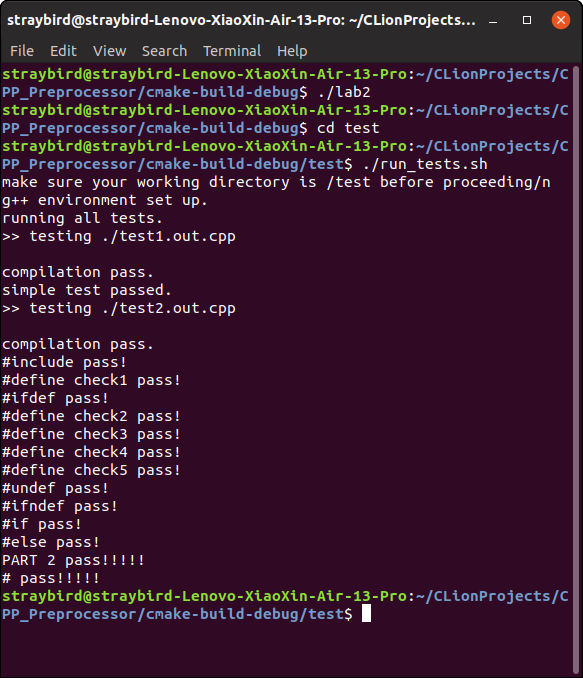
\includegraphics[width=12cm]{shell.png}
  \caption{Testcase Result}\label{2}
\end{figure}

\begin{figure}
  \centering
  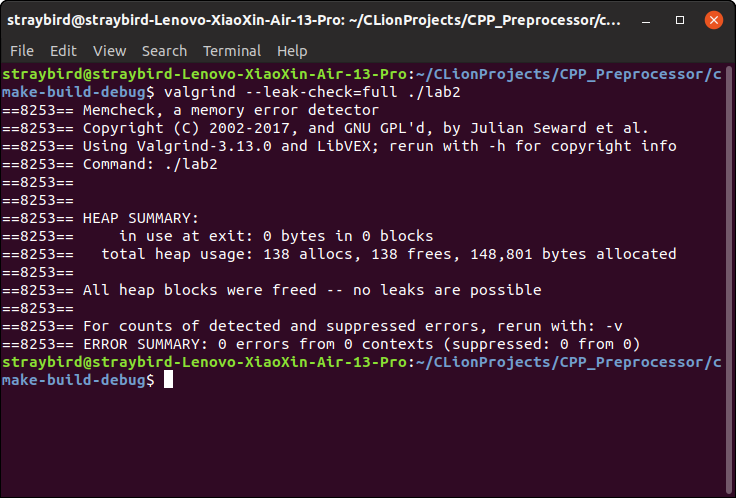
\includegraphics[width=12cm]{mem.png}
  \caption{Memory Leak Check}\label{2}
\end{figure}

\chapter{Memory Leak}
\section{Potential Memory Leak}
\section{Prove of Free from Memory Leak in my Implementation}

\begin{thebibliography}{A}

\bibitem{1}
Wikipedia contributors. (2019, February 3). Encapsulation (computer programming). In \emph{Wikipedia, The Free Encyclopedia}. Retrieved 10:19, March 23, 2019, from \url{https://en.wikipedia.org/w/index.php?title=Encapsulation_(computer_programming)&oldid=881507936}

\bibitem{2}
Wikipedia contributors. (2019, March 17). Reversi. In \emph{Wikipedia, The Free Encyclopedia}. Retrieved 10:20, March 23, 2019, from \url{https://en.wikipedia.org/w/index.php?title=Reversi&oldid=888167585}

\bibitem{3}
Wikipedia contributors. (2019, March 15). Polymorphism (computer science). In \emph{Wikipedia, The Free Encyclopedia}. Retrieved 10:21, March 23, 2019, from \url{https://en.wikipedia.org/w/index.php?title=Polymorphism_(computer_science)&oldid=887878749}

\bibitem{4}
Wikipedia contributors. (2019, February 27). Object-oriented programming. In \emph{Wikipedia, The Free Encyclopedia}. Retrieved 10:22, March 23, 2019, from \url{https://en.wikipedia.org/w/index.php?title=Object-oriented_programming&oldid=885274966}

\bibitem{5}
Wikipedia contributors. (2019, February 21). Inheritance (object-oriented programming). In \emph{Wikipedia, The Free Encyclopedia}. Retrieved 10:22, March 23, 2019, from \url{https://en.wikipedia.org/w/index.php?title=Inheritance_(object-oriented_programming)&oldid=884436146}

\end{thebibliography}
\end{document} 